%%%%%%%%%%%%%%%%%%%%%%%%%%%%%%%%%%%%%%%%%%%%%%%%%%%%%%%%%%%%%%%%%%%%%%
%%                                                                  %%
%%  Pulse Reliability Atlas -- npj Digital Medicine submission      %%
%%                                                                  %%
%%  Maintainer: Santino Nanini                                      %%
%%  Build:      see preprint_npj/build_npj.ps1                      %%
%%  Sync:       paired with ../preprint/manuscript.md via           %%
%%              preprint_npj/paper_to_monograph_map.md and          %%
%%              scripts/audit_claims.py --check-paper-sync          %%
%%  Status:     Step 1 skeleton (abstract + section stubs only).    %%
%%              Subsequent steps draft sections incrementally       %%
%%              per the S028 splitting blueprint.                   %%
%%                                                                  %%
%%%%%%%%%%%%%%%%%%%%%%%%%%%%%%%%%%%%%%%%%%%%%%%%%%%%%%%%%%%%%%%%%%%%%%

\documentclass[pdflatex,sn-nature]{sn-jnl}% Style for submissions to Nature Portfolio journals

%%%% Standard packages (verbatim from upstream Springer Nature sample)
\usepackage{graphicx}%
\usepackage{multirow}%
\usepackage{amsmath,amssymb,amsfonts}%
\usepackage{amsthm}%
\usepackage{mathrsfs}%
\usepackage[title]{appendix}%
\usepackage{xcolor}%
\usepackage{textcomp}%
\usepackage{manyfoot}%
\usepackage{booktabs}%
\usepackage{algorithm}%
\usepackage{algorithmicx}%
\usepackage{algpseudocode}%
\usepackage{listings}%
\usepackage{subcaption}% added Step 3: 2x3 sub-figure layout for Morris mu* heatmaps (Figure 2)
\usepackage{xr-hyper}% Step 10: cross-document references to supplement.tex
\externaldocument{supplement}% reads supplement.aux to resolve \ref{sec:s*}, \ref{fig:s*}, \ref{tab:s*}

\raggedbottom

\begin{document}

%%%%%%%%%%%%%%%%%%%%%%%%%%%%%%%%%%%%%%%%%%%%%%%%%%%%%%%%%%%%%%%%%%%%%%
%% TITLE                                                            %%
%% The active title below is Candidate B (synthetic-cohort framing, %%
%% selected for npj Digital Medicine audience -- digital-health and %%
%% clinical-AI readership). Candidates A and C are preserved as     %%
%% commented alternatives so the maintainer can swap with a         %%
%% one-line edit if reviewer feedback or supervisor input prefers   %%
%% an alternative framing.                                          %%
%%                                                                  %%
%% Candidate A (digital-twin framing, ambitious but uses contested  %%
%% terminology):                                                    %%
%% \title[Reliability atlas: Pulse Physiology Engine]{Mapping the   %%
%%   reliability of an open-source physiological digital twin for   %%
%%   adult critical-care simulation: sensitivity, silent clamping,  %%
%%   and sex-stratified solver divergence in the Pulse Physiology   %%
%%   Engine}                                                        %%
%%                                                                  %%
%% Candidate C (cleanest, methods-paper friendly, less audience     %%
%% hook):                                                           %%
%% \title[Reliability atlas: Pulse Physiology Engine]{A reliability %%
%%   atlas for the Pulse Physiology Engine: operational             %%
%%   sensitivity, silent clamping, and sex-stratified solver        %%
%%   divergence across the adult critical-care envelope}            %%
%%%%%%%%%%%%%%%%%%%%%%%%%%%%%%%%%%%%%%%%%%%%%%%%%%%%%%%%%%%%%%%%%%%%%%

\title[Reliability atlas: Pulse Physiology Engine]{An open reliability atlas for synthetic patient cohorts: sensitivity, divergence, and sex-stratified failure modes in the Pulse Physiology Engine v4.3.1}

%%%%%%%%%%%%%%%%%%%%%%%%%%%%%%%%%%%%%%%%%%%%%%%%%%%%%%%%%%%%%%%%%%%%%%
%% AUTHOR + AFFILIATIONS                                            %%
%% Replicated byte-for-relevant-byte from ../preprint/manuscript.md %%
%% lines 3-19 (after the YAML frontmatter and the Affiliations      %%
%% block). Single corresponding author across four affiliations.    %%
%% Underscore-S in 'UMR_S' escaped as 'UMR\_S'. French accents      %%
%% rendered with LaTeX escapes (\`e, \'e). Street and postcode      %%
%% omitted in \orgaddress because the monograph does not record     %%
%% them; \city / \state / \country are sufficient per sn-jnl.       %%
%%                                                                  %%
%% Corresponding-author primary affiliation: marker on \affil*[4]   %%
%% (CHU Sainte-Justine / Universite de Montreal PICU) per           %%
%% maintainer directive in S028 Step 2 (2026-05-23). Affiliations   %%
%% 1-4 retain their monograph ordering; only the * marker moved.    %%
%%%%%%%%%%%%%%%%%%%%%%%%%%%%%%%%%%%%%%%%%%%%%%%%%%%%%%%%%%%%%%%%%%%%%%

\author*[1,2,3,4]{\fnm{Santino} \sur{Nanini}}\email{santino.nanini@umontreal.ca}

\author[5]{\fnm{Yassir} \sur{Mamouni}}

\author[5]{\fnm{Philippe} \sur{Jouvet}}

\author[5]{\fnm{Cyril} \sur{Schweitzer}}

\author[5]{\fnm{Arnaud} \sur{Wiedemann}}

\author[5]{\fnm{Michael} \sur{Sauthier}}

\affil[1]{\orgdiv{INSERM UMR\_S 1256, Nutrition, Genetics, and Environmental Risk Exposure}, \orgname{University of Lorraine, Faculty of Medicine of Nancy}, \orgaddress{\country{France}}}

\affil[2]{\orgdiv{Research Center}, \orgname{Sainte-Justine University Hospital}, \orgaddress{\city{Montreal}, \state{Quebec}, \country{Canada}}}

\affil[3]{\orgdiv{Clinical Decision Support System Artificial Intelligence Health Cluster in Acute Child Care (PE-DIATRICS)}, \orgname{CHU Sainte-Justine Centre Hospitalier Universitaire M\`ere-Enfant}, \orgaddress{\city{Montr\'eal}, \country{Canada}}}

\affil*[4]{\orgdiv{Pediatric Intensive Care Unit, Department of Pediatrics}, \orgname{CHU Sainte-Justine, Universit\'e de Montr\'eal}, \orgaddress{\city{Montreal}, \state{QC}, \country{Canada}}}

\affil[5]{\orgdiv{[AFFILIATION PLACEHOLDER]}, \orgname{[AFFILIATION PLACEHOLDER]}, \orgaddress{\country{[AFFILIATION PLACEHOLDER]}}}

%%%%%%%%%%%%%%%%%%%%%%%%%%%%%%%%%%%%%%%%%%%%%%%%%%%%%%%%%%%%%%%%%%%%%%
%% ABSTRACT                                                         %%
%% 145 words (target 150, -5 slack). 6 sentences per S028           %%
%% refinement #3. Three headline findings, one number each. Every   %%
%% numerical claim is registered in paper_to_monograph_map.md       %%
%% with its monograph claim_id and expected_occurrences count.      %%
%%%%%%%%%%%%%%%%%%%%%%%%%%%%%%%%%%%%%%%%%%%%%%%%%%%%%%%%%%%%%%%%%%%%%%

\abstract{Pulse is among the most-cited open-source whole-body physiology simulators, used for synthetic patient cohorts and computational physiology research. Yet no formal sensitivity analysis of its operational inputs has been published. We present the first reliability atlas across the adult critical-care envelope: Morris elementary-effects sampling of seven inputs across four Acute Respiratory Distress Syndrome (ARDS) severities and two patient reference bodies (1{,}280 simulations). Tidal-volume instability in 20.6~\% of runs is identified as patient-ventilator dyssynchrony and corrected by setting the volume-controlled assist-control (VC-AC) inspiration trigger to $-2$~cmH$_2$O. A transient hyperoxia regime at FiO$_2$~=~1.0 means 120-second simulations underestimate plateau PaO$_2$; 300-second runs converge to a plateau (median 643~mmHg) sitting $\sim$20~mmHg below the alveolar-gas-equation prediction of $\approx$663~mmHg, consistent with Pulse's modelled A-a gradient. Solver divergence concentrated entirely on the male reference body (20/1{,}280 runs); reducing the male blood-volume baseline toward its 4{,}082.24~mL floor monotonically eliminated divergence. The resulting per-cell traffic-light map provides a reusable data-quality filter for downstream users---including machine-learning and clinical-AI pipelines that rely on such synthetic patient cohorts; all data and code are released open-source under Apache-2.0.}

\keywords{Pulse Physiology Engine, sensitivity analysis, digital twin, synthetic patient data, ICU simulation, Morris elementary effects, reproducibility, ARDS, machine learning training data, operational envelope, computational physiology}

\maketitle

%%%%%%%%%%%%%%%%%%%%%%%%%%%%%%%%%%%%%%%%%%%%%%%%%%%%%%%%%%%%%%%%%%%%%%
%% SECTION SKELETONS                                                %%
%% Each subsection is a stub. Subsequent S028 Steps draft them      %%
%% incrementally per the blueprint. Stubs are LaTeX comments so     %%
%% the rendered PDF shows headings without placeholder prose.       %%
%%%%%%%%%%%%%%%%%%%%%%%%%%%%%%%%%%%%%%%%%%%%%%%%%%%%%%%%%%%%%%%%%%%%%%

\section{Introduction}\label{sec:intro}

The Pulse Physiology Engine (Kitware, Apache-2.0) is among the most actively maintained open-source whole-body human physiology simulators~\cite{bray2019}. It uses a lumped-parameter approach (modelling physiological systems as small networks of coupled compartments rather than full three-dimensional anatomy) to deliver real-time cardiovascular, respiratory, gas-exchange, and pharmacological simulation. Pulse has been applied to ventilator-protocol safety analysis during the COVID-19 pandemic~\cite{webb2020}, to mechanical-ventilator implementation and validation against the ASL 5000 reference~\cite{webb2022vent}, and to external statistical assessment as a digital-twin candidate for retrospective clinical cohorts~\cite{cornish2023}. Across these settings, Pulse generates synthetic patient trajectories that downstream researchers use for hypothesis testing, device validation, and computational physiology studies. Yet despite this footprint, no public sensitivity, divergence, or input-clamping map of Pulse's user-facing operational envelope has been published. Each downstream user re-encounters the same engine limitations independently, and each validation pipeline re-derives its own working envelope by trial and error.

The Pulse maintainers state on the project's public FAQ that ``we have not performed a systematic forward propagation or inverse quantification of model uncertainty, nor have we conducted a formal sensitivity analysis''~\cite{pulsefaq}. The upstream code repository carries a single sensitivity-analysis study, tagged \texttt{STUDY\_SENSITIVITY\_ANALYSIS\_1\_0\_0} (2020), but that study targets internal vascular-circuit resistance multipliers for model calibration --- a different parameter class from the user-facing operational inputs (heart rate (HR), systolic and diastolic blood pressure (SBP and DBP), respiratory rate (RR), tidal volume (Vt), inspired oxygen fraction (FiO$_2$), and positive end-expiratory pressure (PEEP)) that downstream applications must specify. The only prior external assessment of Pulse, by Cornish et al.~\cite{cornish2023}, applied a causal-falsification framework to MIMIC-III sepsis trajectories. Their findings identified intervention-outcome inaccuracies concentrating on electrolyte, metabolic, and acid--base outputs, which do not overlap the present atlas's six-output cardio-respiratory panel. The complementary operational-input reliability question --- how Pulse responds across its acceptance envelope when its primary user-facing controls are varied --- has remained unaddressed.

We close this gap with the first open reliability atlas across Pulse's adult critical-care operational envelope. We sweep the same seven user-facing inputs and track six steady-state outputs (HR, mean arterial pressure (MAP), tidal volume delivered, peripheral oxygen saturation (SpO$_2$), arterial oxygen partial pressure (PaO$_2$), and arterial carbon dioxide partial pressure (PaCO$_2$)) across four Acute Respiratory Distress Syndrome (ARDS) severity scenarios (healthy baseline through severe ARDS) and two adult reference patient bodies. The sampler is Morris elementary-effects screening~\cite{morris1991,campolongo2007} --- a one-input-at-a-time perturbation design that estimates each input's average influence on each output along randomised trajectories through the input space and flags non-linearity and input--input interaction effects. Every simulation is classified by a four-flag steady-state detector that records whether Pulse silently clamped an out-of-range input, the solver diverged, the steady-state output landed outside hard physiological bounds, or the trajectory failed to settle within the simulation window --- categorizing failures rather than discarding them, so that the resulting atlas remains complete across the full input grid. The atlas surfaces three operator-actionable findings (a volume-controlled assist-control (VC-AC) tidal-volume dyssynchrony correction at the inspiration trigger, a steady-state-window correction for hyperoxia simulation, and a previously uncharacterized sex-stratified solver-divergence cluster with an identified blood-volume mechanism) and a per-cell traffic-light reliability map that downstream Pulse users can apply as a data-quality filter on synthetic patient cohorts. The atlas thus addresses a use case beyond simulation training itself: machine-learning and clinical-AI pipelines that increasingly rely on synthetic patient cohorts---such as those generated by Pulse---where engine reliability boundaries translate directly into training-set data-quality boundaries. Characterising the adult engine's operational envelope is also a methodological prerequisite for ongoing pediatric translation work: pediatric physiological dynamics differ fundamentally from adult dynamics, so any pediatric adaptation of Pulse must first establish where the adult engine itself is trustworthy. The pipeline is preregistered, fully reproducible from a single Docker image with a fixed seed, and released open-source under Apache-2.0.

\section{Results}\label{sec:results}

\begin{table}[!h]
\centering
\caption{Terms used in this paper. Definitions are stated once here on first use of each term and not repeated in subsequent sections. Section references point to where each term is operationalised.}
\label{tab:terms}
\begin{tabular}{lp{0.75\textwidth}}
\toprule
Term & Definition \\
\midrule
\textbf{Scenario} & One of the four ARDS impairment-fraction settings that fix lung pathology severity: \textbf{S1} healthy baseline (impairment 0.00), \textbf{S2} mild (0.26), \textbf{S3} moderate (0.60), \textbf{S4} severe (0.95). Berlin-definition severity bands (see \S\ref{sec:methods-sweep}). \\
\textbf{Cell} & A single (scenario, sex) slice of the atlas: one of the four scenarios paired with one of the two reference patient bodies (\textbf{M} male, \textbf{F} female), giving $4 \times 2 = 8$ cells per output. Each cell contains 160 simulations. \\
\textbf{Simulation} & One Pulse run at a single point in the 7-dimensional input space, executed for 120~s with the six steady-state outputs sampled every 5~s (Methods \S\ref{sec:methods-sweep}). \\
\textbf{Trajectory} & A radial path through the 7-dimensional input space along which each input is perturbed in turn by one Morris grid step, producing 8 simulations (one baseline plus seven one-input perturbations). 20 trajectories per cell yield $20 \times 8 = 160$ simulations per cell. \\
\textbf{Elementary effect (EE)} & The change in one steady-state output produced by perturbing one input by one Morris grid step at one location along a trajectory, normalised by the perturbation magnitude. Computed per (cell, input, output) from pairs of simulations along the same trajectory. \\
\textbf{$\mu^{*}$} & Mean of the absolute elementary effects of one input on one output across all trajectories in a cell. The Morris input-importance metric reported in Figure~\ref{fig:morris}; large $\mu^{*}$ indicates strong influence of the input on the output in that cell. \\
\textbf{Clean pair} & A pair of simulations along the same trajectory in which \emph{both} endpoints are classified \texttt{clean} by the four-flag detector (no failure flag fired; see \S\ref{sec:methods-detector} for the flag set). Elementary effects are estimated only from clean pairs; pairs with at least one flagged endpoint are excluded. \\
\bottomrule
\end{tabular}
\end{table}

\subsection{Overview of the reliability atlas}\label{sec:results-overview}

The atlas comprises 1{,}280 simulations spanning eight cells of 160 runs each, where each \textit{cell} is a unique pairing of one ARDS severity scenario --- S1 (healthy baseline), S2 (mild), S3 (moderate), or S4 (severe) --- with one patient sex (male or female), giving the $4 \times 2 = 8$ cells. Each simulation is classified by a four-flag steady-state detector: \texttt{clamped} flags whether Pulse silently bent any setup input out of its acceptance band; \texttt{diverged} flags solver failure or non-finite output; \texttt{implausible} flags steady-state means that fall outside hard physiological bounds (e.g.\ PaO$_2$ above 600~mmHg or SpO$_2$ below 50~\%); and \texttt{not\_steady\_state} flags runs whose final 60-second window fails preregistered drift or variance thresholds. The four flags are independent presence counts (a single run can fire several), and Table~\ref{tab:flag_summary} reports the per-cell breakdown.

Three features of Table~\ref{tab:flag_summary} are immediately load-bearing. First, silent clamping never occurs (0 / 1{,}280 across every cell), confirming that Pulse rejects out-of-range inputs loudly rather than silently bending them. Second, solver divergence is sex-stratified: 20 / 1{,}280 runs (1.6~\%) diverged, and all 20 fell on the male reference body (the mechanism is the subject of \S\ref{sec:results-sex}). Third, \texttt{not\_steady\_state} concentrates on healthy adults (S1, where input tidal-volume swings outpace Pulse's VC-AC controller) and on severe ARDS (S4, where the locked simulation window is insufficient for slow convergence under near-shunt physiology) --- both regimes are characterised in \S\ref{sec:results-vcac} and \S\ref{sec:results-hyperoxia}. Across the full sweep, 663 of 1{,}280 simulations (51.8~\%) are flag-clean under the locked classifier; the per-cell reliability traffic-light map (Figure~\ref{fig:traffic_light}) summarises the resulting reliability picture at a glance.

\begin{table}[h]
\centering
\caption{Per-cell flag breakdown across the 8 (scenario $\times$ sex) cells (160 simulations per cell, 1{,}280 total). Flag columns are independent presence counts: a single run can fire several flags simultaneously, so row sums exceed \texttt{n\_total} when runs trigger multiple non-priority flags. Only the \texttt{clean} column is mutually exclusive of the four flag classes. The detector's priority order (\texttt{clamped > diverged > implausible > not\_steady\_state > clean}) is used to resolve runs to a single primary flag for partition-style analyses. Cell-label key (Table~\ref{tab:terms}): S1 healthy baseline, S2 mild ARDS, S3 moderate, S4 severe; \_M and \_F denote the male and female reference body.}
\label{tab:flag_summary}
\begin{tabular}{lrrrrrr}
\toprule
Cell & n\_total & clamped & diverged & implausible & not\_steady\_state & clean \\
\midrule
S1\_M & 160 & 0 & 4 & 11 & 107 & 49 \\
S1\_F & 160 & 0 & 0 & 23 & 118 & 42 \\
\midrule
S2\_M & 160 & 0 & 4 & 0  & 69  & 87 \\
S2\_F & 160 & 0 & 0 & 0  & 68  & 92 \\
\midrule
S3\_M & 160 & 0 & 4 & 0  & 12  & 144 \\
S3\_F & 160 & 0 & 0 & 0  & 38  & 122 \\
\midrule
S4\_M & 160 & 0 & 8 & 46 & 44  & 67 \\
S4\_F & 160 & 0 & 0 & 46 & 74  & 60 \\
\bottomrule
\end{tabular}
\end{table}

\begin{figure}[h]
\centering
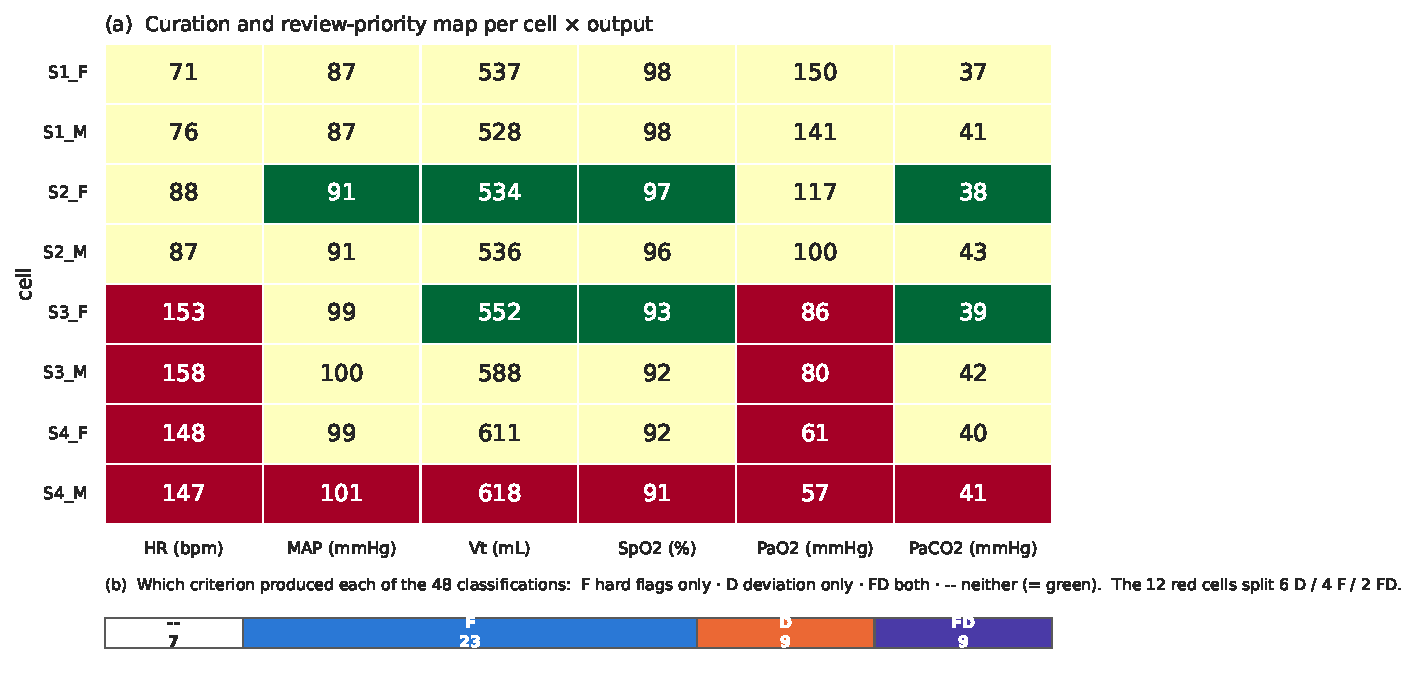
\includegraphics[width=0.95\textwidth]{figures/fig01_traffic_light.pdf}
\caption{Per-cell reliability traffic-light map across the 8 (scenario $\times$ sex) cells and the 6 steady-state outputs (HR, mean arterial pressure (MAP), Vt delivered, SpO$_2$, PaO$_2$, PaCO$_2$). Cells are coloured \textit{green} when no diverged or implausible flags are raised \textit{and} the clean-run mean lies within $10~\%$ of the (S1, M) baseline; \textit{yellow} when any diverged or implausible flag is raised \textit{or} the mean is $10$--$30~\%$ off baseline; \textit{red} when the mean is more than $30~\%$ off baseline \textit{or} the diverged-plus-implausible rate exceeds $30~\%$. The aggregate breakdown is 7 green / 29 yellow / 12 red across the 48 cell $\times$ output combinations. Cell-label key (Table~\ref{tab:terms}): S1 healthy baseline, S2 mild ARDS, S3 moderate, S4 severe; \_M and \_F denote the male and female reference body.}
\label{fig:traffic_light}
\end{figure}

\subsection{Primary input-sensitivity rankings}\label{sec:results-morris}

Figure~\ref{fig:morris} shows the Morris $\mu^{*}$ (mean of absolute elementary effects, the input-importance metric) for each of the six outputs across the eight cells and the seven swept inputs. The preregistered first hypothesis was that, in every cell, the top-three inputs account for at least 50~\% of summed $\mu^{*}$ on each output --- a ``skewed sensitivity'' criterion that determines whether a small subset of inputs explains most of the output variability. The data support this on 48 of 48 cell $\times$ output combinations, with a median top-3 fraction of 0.928 (range 0.658--0.998) under a 1{,}000-resample bootstrap confidence interval.

Four cross-output patterns emerge directly from Figure~\ref{fig:morris} (full per-cell tables in Supplement~\S\,\ref{sec:s3}). Cardiovascular outputs are cardio-input dominated: output HR is driven by input HR in every cell, and output MAP is driven by SBP in every cell, with no measurable cross-talk from ventilator settings. Gas-exchange outputs are ventilator-driven. PaO$_2$ is dominated by FiO$_2$ in S2 / S3 (mild and moderate ARDS) and collapses to a near-flat dependence in S4 (severe ARDS), correctly reproducing the textbook ARDS regime in which shunt physiology pins arterial oxygenation independent of inspired oxygen. PaCO$_2$ is dominated by tidal volume in most cells, consistent with the alveolar-ventilation identity $\dot{V}_A = \mathrm{RR} \cdot (V_T - V_D)$. Output Vt tracks input Vt at far higher $\mu^{*}$ magnitudes than any other input--output pair, reflecting the near-deterministic coupling of VC-AC ventilation outside the dyssynchrony regime described in \S\ref{sec:results-vcac}. SpO$_2$ shows the smallest $\mu^{*}$ magnitudes overall because the output sits at the hemoglobin-saturation ceiling across most of the swept range. The lowest top-3 fractions all fall in severe-ARDS gas-exchange cells (S4\_F SpO$_2$ at 0.658, S4\_M SpO$_2$ at 0.703), where the saturation ceiling distributes sensitivity more uniformly across the inputs --- these being the only cells in the atlas where the skewed-sensitivity property weakens.

\begin{figure}[!htbp]
\centering
\begin{subfigure}[b]{0.50\textwidth}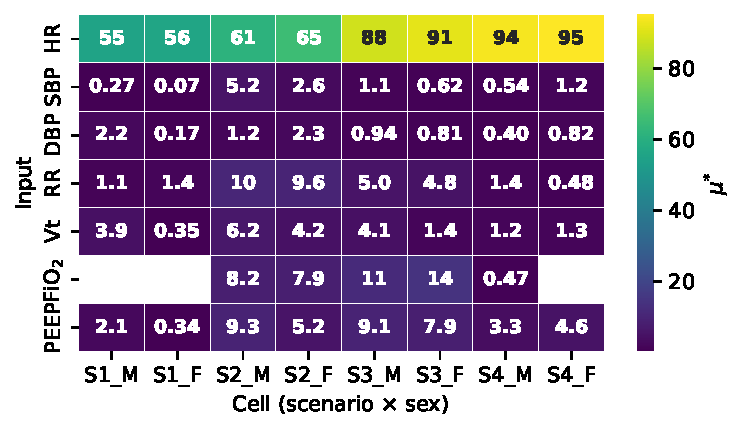
\includegraphics[width=\textwidth]{figures/fig02_morris_HR.pdf}\caption{HR}\label{fig:morris-hr}\end{subfigure}\hfill
\begin{subfigure}[b]{0.50\textwidth}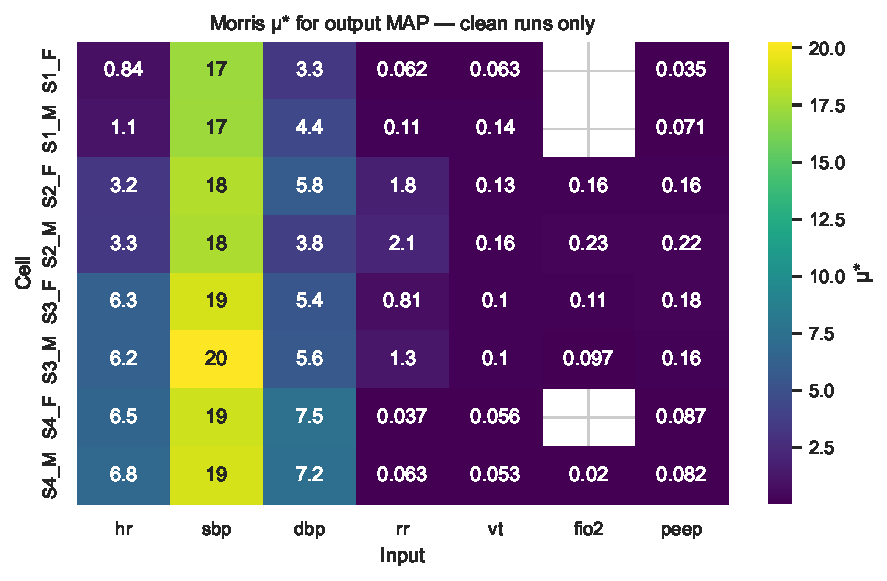
\includegraphics[width=\textwidth]{figures/fig02_morris_MAP.pdf}\caption{MAP}\label{fig:morris-map}\end{subfigure}
\\[0.5em]
\begin{subfigure}[b]{0.50\textwidth}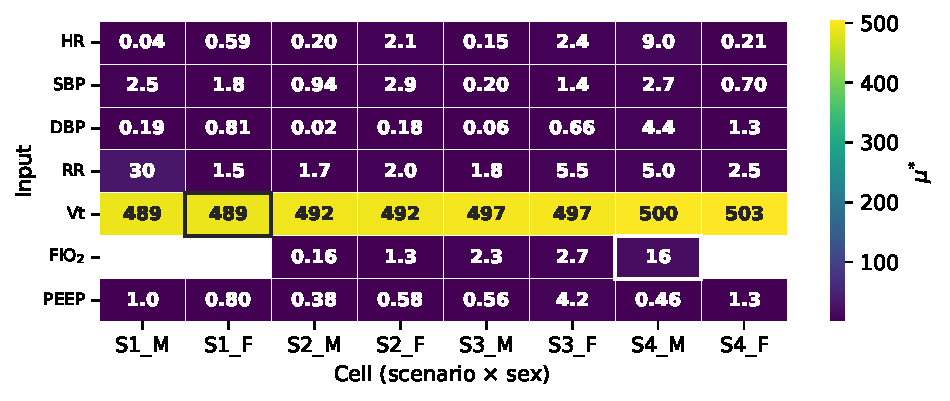
\includegraphics[width=\textwidth]{figures/fig02_morris_Vt.pdf}\caption{Vt delivered}\label{fig:morris-vt}\end{subfigure}\hfill
\begin{subfigure}[b]{0.50\textwidth}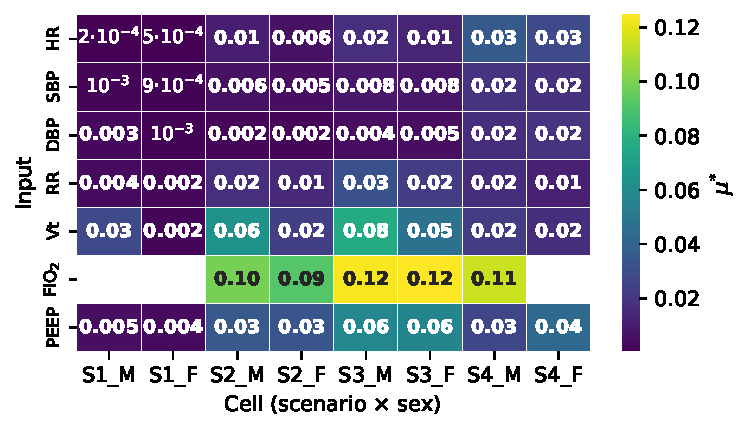
\includegraphics[width=\textwidth]{figures/fig02_morris_SpO2.pdf}\caption{\texorpdfstring{SpO$_2$}{SpO2}}\label{fig:morris-spo2}\end{subfigure}
\\[0.5em]
\begin{subfigure}[b]{0.50\textwidth}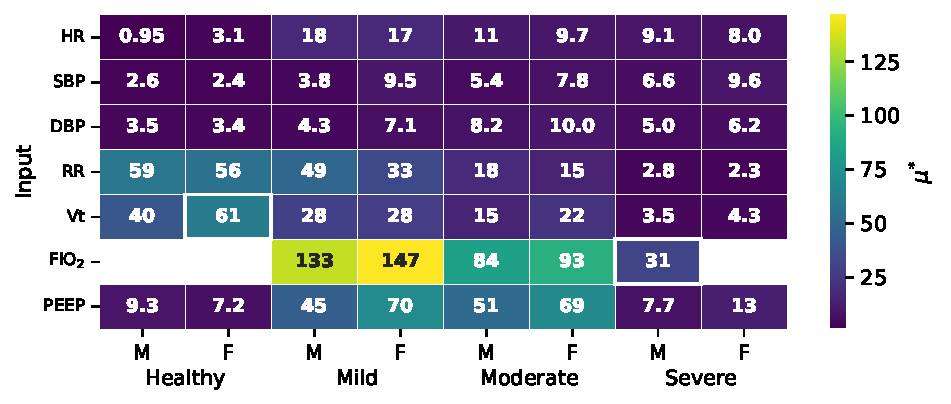
\includegraphics[width=\textwidth]{figures/fig02_morris_PaO2.pdf}\caption{\texorpdfstring{PaO$_2$}{PaO2}}\label{fig:morris-pao2}\end{subfigure}\hfill
\begin{subfigure}[b]{0.50\textwidth}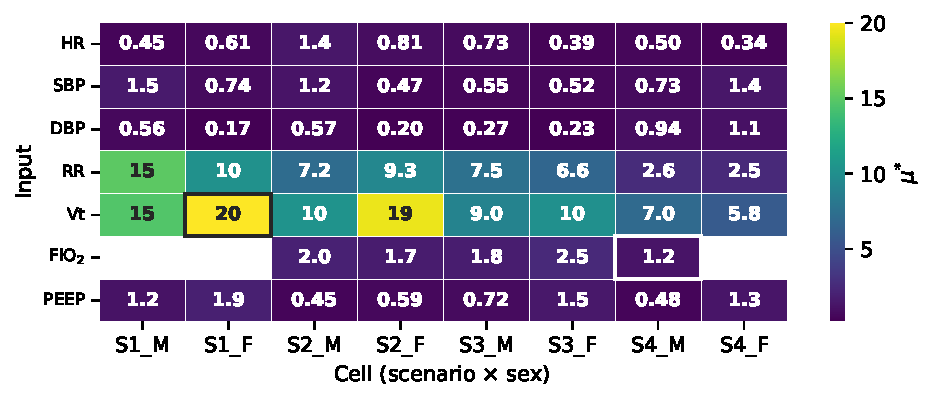
\includegraphics[width=\textwidth]{figures/fig02_morris_PaCO2.pdf}\caption{\texorpdfstring{PaCO$_2$}{PaCO2}}\label{fig:morris-paco2}\end{subfigure}
\caption{Morris $\mu^{*}$ heatmaps for the six steady-state outputs. Rows of each panel are the seven swept inputs (HR, SBP, DBP, RR, Vt, FiO$_2$, PEEP); columns are the eight (scenario $\times$ sex) cells. Colour intensity is the magnitude of the input's mean absolute elementary effect on that output. Cell annotations use plain decimal at standard precision down to $10^{-3}$ (e.g., $55$, $0.27$, $0.005$); below that the compact mathtext form $10^{e}$ is used for pure powers of ten and $m{\cdot}10^{e}$ otherwise (e.g., $9{\cdot}10^{-4}$). This keeps every cell within four digits and is only visually relevant for SpO$_{2}$, the only output whose $\mu^{*}$ range reaches that low. The visual diagonal pattern in each panel supports Hypothesis 1's ``skewed sensitivity'' claim (top-3 inputs explain $\geq 50~\%$ of summed $\mu^{*}$ on 48 of 48 cell $\times$ output combinations, median 0.928). Cell-label key (Table~\ref{tab:terms}): S1 / S2 / S3 / S4 = healthy / mild / moderate / severe ARDS; \_M / \_F = male / female reference body.}
\label{fig:morris}
\end{figure}

\subsection{\texorpdfstring{VC-AC tidal-volume dyssynchrony and the $-2$~cmH$_2$O fix}{VC-AC tidal-volume dyssynchrony and the -2 cmH2O fix}}\label{sec:results-vcac}

The largest contributor to the \texttt{not\_steady\_state} flag count across the full sweep is tidal-volume oscillation under volume-controlled assist-control ventilation. Within the locked 120-second simulation window, the delivered tidal-volume coefficient of variation (Vt CV, the standard deviation of breath-by-breath delivered Vt divided by its mean over the final 60-second steady-state window) exceeds the 0.05 detector threshold on 20.6~\% of runs (Figure~\ref{fig:corrections}a, x-axis distribution). The pattern is concentrated on healthy adults (visible as the elevated S1 \texttt{not\_steady\_state} counts in Table~\ref{tab:flag_summary}) and fades as ARDS severity increases, consistent with a patient-ventilator-trigger interaction that activates when respiratory drive is high and lung compliance is normal --- a clinically documented form of patient-ventilator asynchrony~\cite{figueroacasas2016} rather than a Pulse-specific solver artefact.

We preregistered a follow-up experiment that isolated the mechanism. We re-ran 64 of the affected configurations with a single intervention: setting Pulse's \texttt{InspirationPatientTriggerPressure} to $-2$~cmH$_2$O on the \texttt{SEMechanicalVentilatorVolumeControl} action (upstream source: \texttt{SEMechanicalVentilatorVolumeControl.cpp} lines 120--128). This disables the respiratory-model-driven patient trigger and replaces it with a clinically standard intensive-care unit (ICU) sensitivity setting. The intervention collapses the median Vt CV from 0.351 to 0.016 (Figure~\ref{fig:corrections}a, dots well below the diagonal) and reduces the worst-case Vt CV from 1.826 to 0.112; 78.1~\% of locked-trigger reruns drop below the 0.05 steady-state threshold, satisfying both preregistered acceptance gates.

The practical consequence for downstream Pulse users is direct: any VC-AC sensitivity study or virtual-cohort generation that requires deterministic tidal-volume delivery should set \texttt{InspirationPatientTriggerPressure} explicitly to $-2$~cmH$_2$O (or another clinically standard value) on every action. Without this setting, Pulse's default VC-AC behaviour produces realistic patient-ventilator asynchrony at exactly the ventilator-stress points where validation matters most --- physiologically faithful, but not steady-state interpretable under the conventional final-60-second window.

\subsection{\texorpdfstring{Transient hyperoxia regime at FiO$_2$~=~1.0}{Transient hyperoxia regime at FiO2 = 1.0}}\label{sec:results-hyperoxia}

A second cluster of preregistered detector flags concentrates on the highest inspired-oxygen settings. Within the locked 120-second simulation window, Pulse's steady-state mean PaO$_2$ exceeds the detector's locked upper bound of 600~mmHg on 34 of the 126 \texttt{implausible}-flagged runs, and 91~\% of these excursions occur at FiO$_2 \geq 0.95$. Two competing hypotheses fit this pattern. \textbf{Hypothesis A} --- Pulse is over-delivering oxygenation at the FiO$_2 = 1.0$ boundary (an engine defect). \textbf{Hypothesis B} --- the locked 120-second window is shorter than Pulse's PaO$_2$ relaxation time when shunt physiology is minimal and the alveolar partial pressure is climbing toward its theoretical ceiling (a window-length artefact rather than an engine defect).

A preregistered 60-run extended-simulation experiment discriminated between the two. Each rerun resumed from Pulse's saved engine state at the end of the original 120-second run and continued for an additional 300 seconds, with the plateau computed from the final 60 seconds of the extension (Supplement~\S\,\ref{sec:s9}). In the S1 (healthy) cohort, 41 of 44 reruns (93.2~\%) converged to a stable plateau under the preregistered drift criterion (Figure~\ref{fig:corrections}b, S1 cluster); the converged S1 plateau median was 643~mmHg, sitting approximately 20~mmHg \emph{below} the simple alveolar-gas-equation prediction at sea level of $\approx$~663~mmHg (FiO$_2 = 1.0$, $P_B = 760$, $P_{\mathrm{H_2O}} = 47$, $\mathrm{PaCO}_2 = 40$, $R = 0.8$)~\cite{west2020respiratory}. The $\approx$~20~mmHg gap is consistent with Pulse's modelled alveolar-arterial difference rather than an oxygenation defect, which would be expected to push PaO$_2$ \emph{above} the theoretical ceiling, not below it. The S3 and S4 reruns (Figure~\ref{fig:corrections}b, orange and red clusters) sit far below the 600~mmHg classifier bound, in the physiologically expected range for moderate and severe ARDS at FiO$_2 = 1.0$.

The practical consequence is again direct: hyperoxia studies on Pulse should be simulated for at least 300 seconds before extracting a steady-state plateau. The 120-second window remains adequate for cardiovascular and ventilation outputs (Supplement~\S\,\ref{sec:s9}) but not for oxygenation outputs at the FiO$_2 = 1.0$ extreme, where slow relaxation to the alveolar ceiling drives the apparent excursion above the conservative locked classifier bound. Downstream users should additionally avoid Vt $\times$ RR combinations exceeding $\sim$12~L/min minute ventilation on healthy lungs at FiO$_2 = 1.0$, where extended-window simulations enter a separate solver-instability regime (full characterisation in the companion technical monograph).

\begin{figure}[h]
\centering
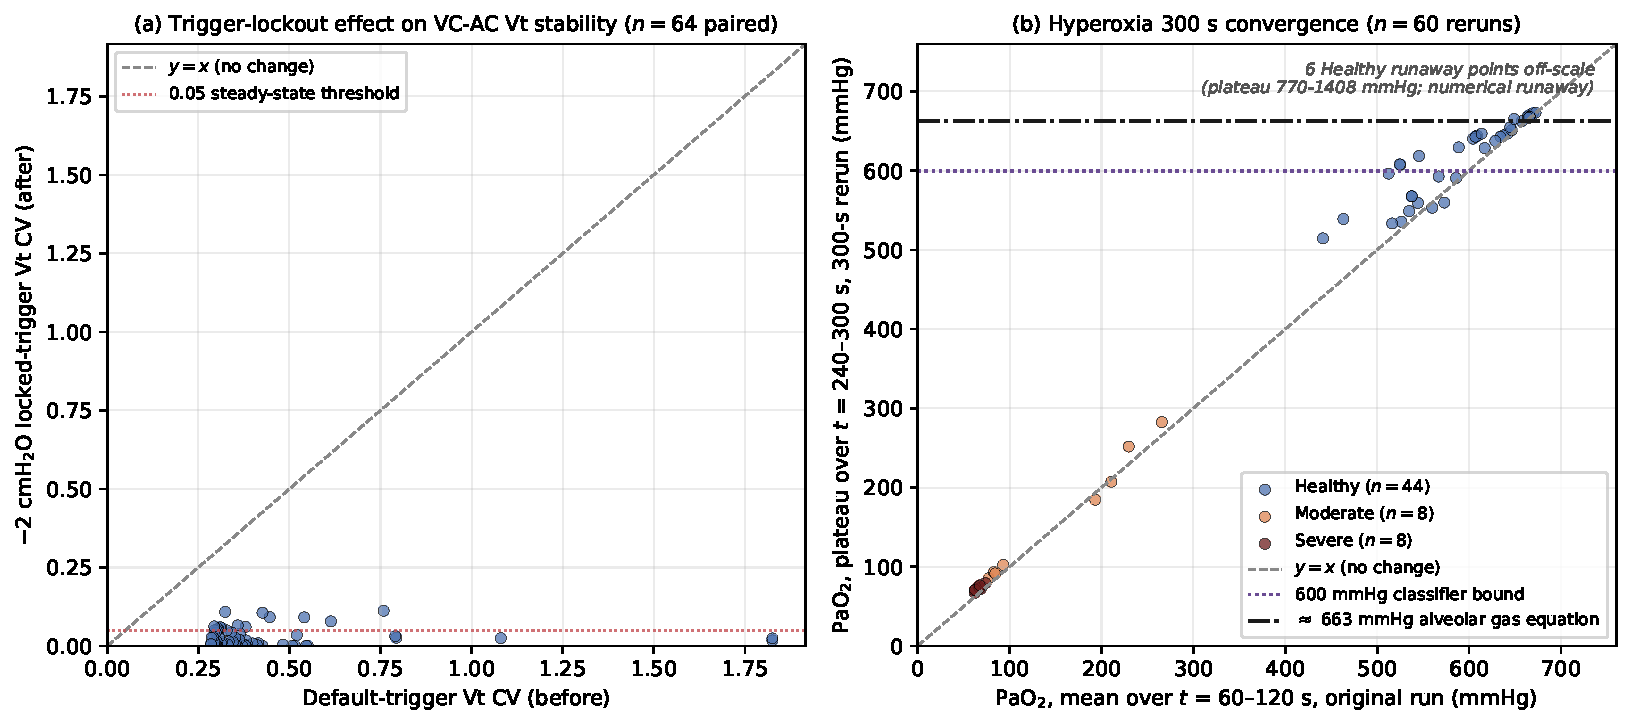
\includegraphics[width=0.95\textwidth]{figures/fig03_actionable_corrections.pdf}
\caption{Two operator-actionable corrections surfaced by the atlas. \textbf{(a)} Trigger-lockout intervention on VC-AC tidal-volume stability ($n = 64$ paired reruns). Each dot is one configuration; the $x$-axis is the original Vt CV under Pulse's default trigger configuration, the $y$-axis is the Vt CV after setting \texttt{InspirationPatientTriggerPressure} to $-2$~cmH$_2$O. The dashed diagonal marks ``no effect'', the dotted horizontal at $0.05$ is the steady-state detector threshold. Median CV collapses from 0.351 to 0.016; 78.1~\% of locked reruns drop below the threshold. \textbf{(b)} Hyperoxia 300-second convergence ($n = 60$ reruns across S1, S3, S4 at FiO$_2 = 1.0$). Each dot is one configuration; the $x$-axis is the original 120-second mean PaO$_2$, the $y$-axis is the 300-second plateau PaO$_2$. The dashed diagonal marks ``no change'', the dotted horizontal at 600~mmHg is the locked classifier upper bound, the dash-dotted horizontal at $\approx$~663~mmHg is the alveolar-gas-equation sea-level prediction. Both panel axes are restricted to the physiological range $[0, 760]$~mmHg to highlight the convergence structure; six S1 reruns develop a numerical runaway and plateau off-scale (up to $\approx$1{,}408~mmHg, Supplement~\S\,\ref{sec:s9}) and are omitted from the visible range. The bulk of the S1 cluster sits just below the prediction, consistent with a transient hyperoxia regime rather than an oxygenation overshoot. Scenario key (Table~\ref{tab:terms}): S1 healthy baseline, S3 moderate ARDS, S4 severe ARDS.}
\label{fig:corrections}
\end{figure}

\subsection{Sex-stratified solver divergence and blood-volume mechanism}\label{sec:results-sex}

Across the full 1{,}280-run sweep, solver divergence is rare but strikingly sex-stratified. 20 runs (1.6~\%) failed to complete with finite output, and \emph{all 20 fell on the male reference body}: 4 in each of S1\_M, S2\_M, S3\_M and 8 in S4\_M, with zero divergences across the 640 runs on the female reference body (Figure~\ref{fig:sex_bv}a). The 20 divergence events are not spread uniformly through the input space. 16 of them concentrate on a specific compound input pattern --- low cardiovascular output (HR = 50, SBP = 90) combined with high respiratory rate (RR = 20) --- a clinically recognisable hypotensive--tachypneic configuration. The FiO$_2 = 1.0$ boundary co-occurs in 13 of the 20 cases. Identical Morris input grids submitted to the female reference body (matched on age, condition string, and ventilator settings; differing only in patient mass, height, and sex flag) never trigger the same numerical edge case.

A preregistered follow-up experiment isolated the mechanism. Pulse's \texttt{SetupPatient.cpp} computes blood-volume baseline by the allometric relation $\text{BV} = 65.6 \cdot \text{weight}_{\text{kg}}^{1.02}$, yielding 4{,}802.63~mL for the 67.3~kg male reference body and 3{,}996.09~mL for the 56.2~kg female body --- a 17~\% sex gap that propagates into the cardiovascular circuit's operating point. We re-executed the 20 originally-diverged male inputs with an explicit \texttt{BloodVolumeBaseline} override at three levels: the default (4{,}802.63~mL), an intermediate bracket (4{,}400~mL, a 8.4~\% reduction), and the engine's setup-time minimum for this body (4{,}082.24~mL, a 15.0~\% reduction). The divergence count fell monotonically: 20 / 20 $\rightarrow$ 2 / 20 $\rightarrow$ 0 / 20 (Figure~\ref{fig:sex_bv}b). Reducing male BV toward the female-equivalent range eliminates the divergence cluster.

A separate engine-level observation emerged from the same experiment: Pulse enforces a hard per-patient floor on \texttt{BloodVolumeBaseline} at setup time --- 4{,}082.24~mL on this male body. Setting BV below the floor triggers an explicit \texttt{[ERROR]} and exit. The practical consequence for sex-comparison studies is that the female-computed BV (3{,}996.09~mL) sits 86~mL below the male floor, so the two reference bodies cannot be made BV-equivalent by a one-way transplant; a true sex-balanced synthetic cohort requires more than just patient-attribute matching. For downstream Pulse users training models on synthetic patient cohorts, the operational implication is concrete: pooling male and female runs from the input-extreme regime without flag-stratified filtering will introduce a hidden sex covariate at the male reference body's divergence boundary --- a structural artefact of Pulse's allometric BV baseline rather than a clinical phenomenon.

\begin{figure}[h]
\centering
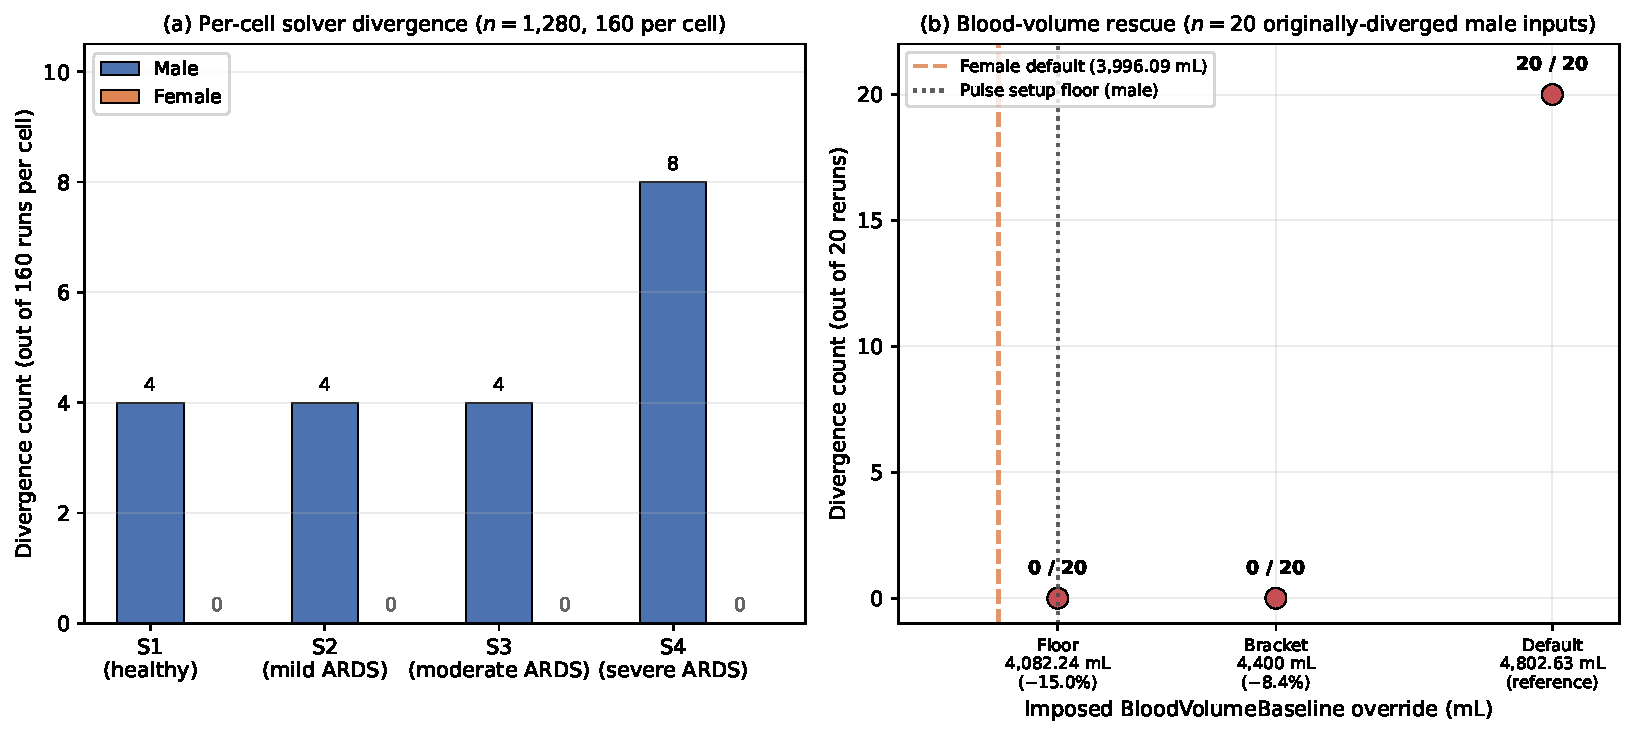
\includegraphics[width=0.95\textwidth]{figures/fig04_sex_bv_mechanism.pdf}
\caption{Sex-stratified solver divergence and its blood-volume mechanism. \textbf{(a)} Divergence counts per (scenario $\times$ sex) cell across the 1{,}280-run sweep. All 20 divergence events fall on the male reference body; the female reference body runs an identical Morris input grid without a single divergence. \textbf{(b)} Blood-volume rescue dose-response on the 20 originally-diverged male inputs. The $x$-axis is the imposed \texttt{BloodVolumeBaseline} override (4{,}802.63~mL default, 4{,}400~mL intermediate bracket, 4{,}082.24~mL Pulse setup-time floor on this body); the $y$-axis is the divergence count out of 20. Pulse's allometric formula computes 3{,}996.09~mL for the female reference body, indicated by the dashed vertical line --- 86~mL below the male floor, so a one-way BV transplant cannot make the two reference bodies BV-equivalent. The monotonic decrease (20 $\rightarrow$ 2 $\rightarrow$ 0) confirms blood-volume baseline as the load-bearing mechanism behind the all-male divergence cluster. Cell-label key in (a) (Table~\ref{tab:terms}): S1 healthy baseline, S2 mild ARDS, S3 moderate, S4 severe; \_M and \_F denote the male and female reference body.}
\label{fig:sex_bv}
\end{figure}

\subsection{Secondary observations}\label{sec:results-secondary}

Three additional findings sit at the boundary of the headline scope but matter for downstream interpretation. Each is summarised here in compact form and fully expanded in the Supplementary Information.

\textbf{First public characterisation of an ARDS impairment-fraction solver-instability band.} Pulse's own methodology documents ARDS severity as a continuous parameter on $[0, 1]$ and exemplifies the range with the round-tenths convention $\{0.0, 0.3, 0.6, 0.9, 1.0\}$; published Pulse validation work and HowTo examples sample at most up to severity 0.9 and do not examine impairment fractions inside the interval 0.91--0.945. Three converging boundary probes within the companion technical work (full provenance in Supplement~\S\,\ref{sec:s5}) first identified 0.91--0.945 as a numerical bifurcation in the respiratory solver, and the present atlas's 200-run continuous-severity sweep at midrange Morris inputs (Supplement~\S\,\ref{sec:s5}) extends the empirical band to $[0.879, 0.945]$ on the low edge and resolves two divergence regimes: an \emph{input-driven} regime concentrated on the male reference body at hypotensive--tachypneic--FiO$_2$~=~1.0 inputs (\S\ref{sec:results-sex}), and a \emph{severity-driven} regime in which both sexes diverge at midrange inputs across $[0.879, 0.945]$. The locked sweep places severe ARDS (S4) at impairment-fraction 0.95, intentionally above this band; downstream Pulse users should avoid $[0.879, 0.945]$ when stable steady-state outputs are required.

\textbf{Compensatory tachycardia decouples input HR from output HR under hypoxemia.} In S1 (healthy), output HR settles near a physiological norm (73.8~bpm mean, $\sigma = 20.4$~bpm across clean runs) regardless of the input HR baseline. By S3 and S4, output HR rises to 155.7~bpm and 147.1~bpm respectively, despite inputs drawn from the same [50, 110]~bpm range --- a substantial sympathetic overshoot driven by Pulse's modelled baroreceptor and chemoreceptor reflexes responding to severe hypoxemia. The compensation is strong enough to override the explicit input baseline, which has direct consequences for machine-learning pipelines: models trained on Pulse synthetic cohorts will internalise this reflex as a steady-state feature rather than an active physiological response (Supplement~\S\,\ref{sec:s15}).

\textbf{Complementarity with prior external falsification work on MIMIC-III.} Cornish et al.~\cite{cornish2023} applied a causal-falsification framework to Pulse on MIMIC-III sepsis trajectories and reported 85 total Hoeffding-inequality rejections across 15 physiological quantities. Of these, 82 of 85 fall outside the four-channel overlap (HR, MAP, PaO$_2$, PaCO$_2$): 80 on channels the present atlas does not assess (electrolyte, metabolic, acid--base, dermal), plus 2 on partial-overlap pressure channels; only 3 of 85 fall on the four-channel overlap, all on PaCO$_2$. The two papers' failure surfaces are therefore complementary rather than redundant: Cornish covers chemistry-and-thermoregulation outputs under clinical-intervention sequences on a real cohort; the present atlas covers cardio-respiratory outputs across the theoretical operational acceptance envelope. The natural follow-up that neither paper does is a metabolic-and-renal atlas sweeping Pulse's endocrine and electrolyte sub-models the way this paper sweeps the cardiopulmonary inputs (Supplement~\S\,\ref{sec:s7}).

\section{Discussion}\label{sec:discussion}

This work delivers the first open, preregistered reliability atlas for the Pulse Physiology Engine across the adult critical-care operational envelope. Three operator-actionable findings emerge from the 1{,}280-run sweep. \textbf{First}, a one-line configuration fix for VC-AC tidal-volume dyssynchrony (\S\ref{sec:results-vcac}). \textbf{Second}, a steady-state-window correction for hyperoxia simulation at FiO$_2 = 1.0$ (\S\ref{sec:results-hyperoxia}). \textbf{Third}, a previously uncharacterised sex-stratified solver-divergence cluster with an identified blood-volume mechanism (\S\ref{sec:results-sex}). The accompanying per-cell traffic-light reliability map (Figure~\ref{fig:traffic_light}) is the principal deliverable for downstream Pulse users: it summarises which combinations of patient reference body, ARDS severity, and steady-state output are trustworthy as-is, which require flag-stratified handling, and which warrant per-channel justification before being ingested into downstream analyses.

For the computational-physiology community, the atlas matters in two ways. First, it directly addresses the Pulse maintainers' own statement that no formal sensitivity or uncertainty quantification has been performed on user-facing operational inputs~\cite{pulsefaq}. Second, the methodology --- Morris elementary-effects screening of operational inputs, combined with a four-flag steady-state classifier that categorises rather than discards every run --- is transferable. No comparable open atlas exists for sibling lumped-parameter engines such as BioGears or HumMod. The recipe demonstrated here on Pulse v4.3.1 can be applied to those engines with engine-specific I/O wrapping, and would meaningfully extend the community's collective reliability picture for synthetic-physiology infrastructure as a whole.

For machine-learning pipelines that train on Pulse-generated synthetic patient cohorts, the four-flag classifier doubles as a per-cell data-quality contract. Green cells in Figure~\ref{fig:traffic_light} are safe to ingest; yellow cells should be filtered to the clean subset with the per-cell flag rate reported in training-set metadata; red cells require per-channel and per-input justification. Two specific traps documented here merit explicit attention. The sex-stratified divergence cluster (\S\ref{sec:results-sex}) means that pooling male and female runs from the input-extreme regime without flag-stratified filtering ingests a hidden sex covariate at the male reference body's divergence boundary --- a structural artefact of Pulse's allometric blood-volume baseline rather than a clinical phenomenon. The compensatory tachycardia decoupling reported in \S\ref{sec:results-secondary} means that input HR and output HR are not interchangeable in ARDS scenarios: models trained on Pulse cohorts will otherwise internalise the engine's baroreceptor and chemoreceptor reflexes as steady-state features rather than active physiological responses to hypoxemia. The combined cardio-respiratory failure-surface mapped here is also complementary to, rather than redundant with, Cornish et al.'s causal-falsification framework on MIMIC-III sepsis trajectories~\cite{cornish2023}: their work flags chemistry-and-thermoregulation accuracy under real clinical-intervention sequences; this work flags cardio-respiratory reliability across the theoretical operational envelope.

Four scope limits bound the conclusions. (i)~The atlas pins to Pulse v4.3.1 (results apply identically to the build-only v4.3.2 release); newer physiology branches will require re-mapping. (ii)~Patient anatomy is restricted to two standard adult reference reference bodies (male and female); the atlas does not characterise body-mass or height variation within sex. (iii)~The operational envelope is adult-critical-care VC-AC ventilation; pediatric translation, alternative ventilator modes (pressure-controlled, pressure-support), and within-run non-steady-state dynamics are out of scope by construction. (iv)~The Morris elementary-effect estimator requires both endpoints of each one-at-a-time (OAT) input perturbation to pass the four-flag classifier; pairs with at least one flagged endpoint are excluded by construction (\S\ref{sec:methods-detector}). At FiO$_2 = 1.0$ in S1, the FiO$_2$ OAT step pairs a baseline near room air with the maximum inspired-oxygen setting, at which healthy-lung steady-state PaO$_2$ rises toward the alveolar-gas-equation sea-level ceiling of $\approx$~663~mmHg~\cite{west2020respiratory} and reliably exceeds the locked PaO$_2$ upper bound of 600~mmHg (the transient-hyperoxia regime characterised in \S\ref{sec:results-hyperoxia}): the FiO$_2 = 1.0$ endpoint is therefore reliably \texttt{implausible}, and every FiO$_2$ pair drops. At FiO$_2 = 0.21$ and FiO$_2 = 1.0$ in S4\_F, severe-ARDS shunt physiology pins SpO$_2$ at the hemoglobin-saturation ceiling or leaves PaO$_2$ still relaxing toward its plateau within the 120-second window, tripping \texttt{not\_steady\_state} on at least one endpoint of each FiO$_2$ pair. The blank FiO$_2$ rows in the corresponding panels of Figure~\ref{fig:morris} and the restriction of the cross-sex Spearman comparison to S2 and S3 (Supplement~\S\,\ref{sec:s6}) are direct, deterministic consequences of the preregistered implausibility-bound and steady-state-window contract applied at the operational envelope's edges --- not a Pulse defect. Additional trajectories would not recover the dropped pairs: the per-pair drop rule applies to every trajectory identically, and the underlying physiology (alveolar-gas equation on healthy lungs at FiO$_2 = 1.0$; shunt-dominated gas exchange in severe ARDS) is the same on every run. Each of these is bounded rather than open-ended; none undermines the atlas's reliability claims within its declared scope.

The reliability atlas presented here is intended as foundational infrastructure rather than a terminal deliverable. The four-flag classifier and the per-cell traffic-light are reusable instruments that downstream Pulse users can apply to their own configurations without re-running the present sweep, and the atlas pipeline (preregistered, reproducible from a single Docker image with a fixed seed, released under Apache-2.0 alongside an audit ledger of all quantitative claims~\cite{wilkinson2016, munafo2017}) is designed to be re-executable when Pulse releases new physiology branches. Three concrete extensions are immediate priorities. The present adult-envelope characterisation is the methodological prerequisite for a pediatric translation layer (in preparation, validation underway), because pediatric physiological dynamics differ fundamentally from adult dynamics and cannot be safely adapted from an unmapped substrate. A native pediatric Pulse fork (planned) follows from that translation work. A complementary metabolic-and-renal atlas would cover the channels Cornish et al.~\cite{cornish2023} identified as most assessment-sensitive but that no operational-input sweep currently characterises. Together, these would broaden the cardiopulmonary-and-metabolic Pulse-reliability picture that the present work begins.

\section{Methods}\label{sec:methods}

\subsection{Pulse engine and configuration}\label{sec:methods-pulse}

All simulations used Pulse v4.3.1 (Kitware, Apache-2.0)~\cite{bray2019}, a real-time-capable lumped-parameter whole-body physiology engine that solves the coupled cardiovascular, respiratory, gas-exchange, endocrine, renal, and drug sub-models as a system of ordinary differential equations at a 20~ms fixed timestep. The respiratory sub-model is a 5-compartment lung (carina, left and right anatomic dead space, left and right alveoli). The engine was executed inside a single \texttt{pulse-atlas-engine} Docker image, pinned for the entire 1{,}280-run sweep so that every simulation runs against bit-identical engine binaries. v4.3.1 was the most recent stable release with documented physiology updates at the time of the sweep; the subsequent v4.3.2 release (August 2025) is build-system-only and contains no physiology, solver, validation, or patient-setup changes, so all atlas results apply identically to v4.3.2 (full release diff in Supplement~\S\,\ref{sec:s1}). The sweep was dispatched to 2--3 parallel Docker workers on commodity laptop hardware, and bit-exact reproduction of the canonical sweep output was verified at three independent layers (the canonical sample, the per-cell aggregate parquets, and the derived statistical artefacts). Mechanical ventilation was restricted to volume-controlled assist-control (VC-AC) mode for cross-run comparability; alternative modes are out of scope by construction.

\subsection{Patient reference bodies}\label{sec:methods-patients}

Two adult reference reference bodies were used: a male body (age 18, 67.3~kg, 180~cm) and a female body (age 18, 56.2~kg, 163~cm). Weights are the U.S.\ Centers for Disease Control and Prevention (CDC) growth-chart 50th-percentile values for 18-year-olds of each sex; heights are clinically standard adult values: the male case fixes the body mass index (BMI) at 20.8 and the female case matches CDC P50 (BMI 21.1) and Pulse's own \texttt{heightStandardFemale\_cm = 163.0} reference. Pulse's setup-time constraints on each reference body --- the blood-volume baseline floor (\S\ref{sec:results-sex}), the systolic/diastolic blood-pressure gate, and the heart-rate / respiratory-rate initialisation bands --- were verified empirically (\S\ref{sec:methods-sweep}) and respected by the sampler so that the Morris design never proposes inputs outside Pulse's accepted envelope.

\subsection{Sweep design}\label{sec:methods-sweep}

Seven user-facing operational inputs were swept across their verified Pulse acceptance ranges: heart rate (HR, 50--110~bpm), systolic and diastolic blood pressure (SBP 90--120~mmHg, DBP 60--80~mmHg with the post-clip pulse-pressure ratio DBP/SBP $\leq 0.75$ enforced), respiratory rate (RR, 8--20~bpm), tidal volume (Vt, 300--800~mL), inspired oxygen fraction (FiO$_2$, 0.21--1.0), and positive end-expiratory pressure (PEEP, 0--20~cmH$_2$O). Mean arterial pressure (MAP) was derived from SBP and DBP as $\mathrm{DBP} + (\mathrm{SBP} - \mathrm{DBP})/3$ rather than swept independently. Four scenarios spanned the adult critical-care severity range: a healthy baseline (S1, ARDS impairment fraction = 0) and three Acute Respiratory Distress Syndrome severities (S2, mild, impairment = 0.26; S3, moderate, impairment = 0.60; S4, severe, impairment = 0.95) calibrated against the Berlin Definition PaO$_2$/FiO$_2$ bands~\cite{ards2012} and bracketing the 0.91--0.945 solver-instability zone characterised in the companion technical work (Supplement~\S\,\ref{sec:s5}). The Morris elementary-effects design~\cite{morris1991, campolongo2007} used 20 trajectories at 4 grid levels per input, generated via SALib~\cite{iwanaga2022} with random seed 42; each trajectory contributes $(\mathrm{num\_inputs} + 1) = 8$ model evaluations, yielding 160 runs per (scenario $\times$ sex) cell and 1{,}280 runs across the full sweep. Each run executed for 120 seconds of simulated time, with output channels sampled at 5-second intervals (13 samples in the final 60-second steady-state window).

\subsection{Steady-state classifier}\label{sec:methods-detector}

Every simulation was classified by a four-flag steady-state detector before any statistical analysis. \texttt{clamped} fires when Pulse's setup-rejection log contains any of 4 documented input-rejection patterns, indicating that Pulse silently bent a setup input out of its acceptance band. \texttt{diverged} fires when the simulation failed to complete with finite output, the CSV is missing, or the engine exited with a non-zero status. \texttt{implausible} fires when any steady-state output mean exceeds the locked hard physiological bounds (representative bounds: HR [20, 220]~bpm, PaO$_2$ [20, 600]~mmHg, SpO$_2$ [50, 100]~\%). The complete bound table is reproduced in Supplement~\S\,\ref{sec:s3}, where each bound is anchored to primary critical-care and respiratory-physiology literature: the ARDS Network lung-protective ventilation trial~\cite{brower2000}, the Severinghaus oxyhemoglobin dissociation curve~\cite{severinghaus1979}, the Sepsis-3 and Surviving Sepsis Campaign hemodynamic thresholds~\cite{singer2016, evans2021sepsis}, the ESH 2023 hypertensive emergency definition~\cite{mancia2023esh}, and West's respiratory physiology~\cite{west2020respiratory}. The PaO$_2$ upper bound of 600~mmHg is deliberately conservative relative to the alveolar-gas-equation sea-level ceiling of $\approx$~663~mmHg on FiO$_2$ = 1.0; a parallel sensitivity-analysis reclassification under the alternative \texttt{HARD\_BOUNDS\_PHYSIOLOGICAL} dictionary (PaO$_2$ upper raised to 700~mmHg) is reported in Section~\ref{sec:results-hyperoxia} and characterised in the companion technical monograph. \texttt{not\_steady\_state} fires when the steady-state output flatlines at a physiological extreme, exhibits variance above the locked coefficient-of-variation threshold (0.05 for tidal volume), or drifts more than the per-channel locked threshold (Supplement~\S\,\ref{sec:s3}) over the final 60-second window, where drift is estimated by ordinary least-squares regression on the 13 sample points in the [60, 120]~s window. The four flags are independent presence counts; a single simulation can fire several. For partition-style analyses the priority order \texttt{clamped > diverged > implausible > not\_steady\_state > clean} resolves each run to a single \texttt{primary\_flag}. A 22-run pilot on the healthy-male cell verified five preregistered gating criteria (success rate, detector self-consistency, 13-point steady-state window, clamp-regex reachability, and Pulse determinism within a $10^{-6}$ relative tolerance) before the full sweep launched; all thresholds were locked in preregistration before any data was collected~\cite{munafo2017}.

The [60, 120]~s steady-state window itself was preregistered before any sweep data was collected. Pulse settles within $\sim$~45~s under VC-AC (verified empirically in the companion technical work), so opening the evaluation window at $t = 60$~s leaves a $\geq 15$~s margin past settle, and 13 sample points at the 5-second interval are the minimum that resolve the OLS-slope, coefficient-of-variation, and flatline diagnostics that gate the \texttt{not\_steady\_state} flag. A cross-output audit on the full sweep (companion technical work, S012) verifies that drift above the locked per-channel thresholds is contained at 2.6~\% for HR, 0.7~\% for MAP, and 2.0~\% for PaCO$_2$ across the union of the F-003 hyperoxia, F-004 Vt-oscillation, and dual-vulnerability populations; the only exception --- PaO$_2$ and Vt at FiO$_2 \geq 0.95$ --- is the transient hyperoxia regime fully characterised in \S\ref{sec:results-hyperoxia}.

\subsection{Statistical analyses}\label{sec:methods-stats}

Morris mean-absolute-elementary-effect indices ($\mu^{*}$) and standard deviations ($\sigma$) were computed per (scenario, sex, input, output) cell using the SALib implementation~\cite{iwanaga2022}, with non-parametric 95~\% bootstrap confidence intervals on $\mu^{*}$ from 1{,}000 trajectory-level resamples. Hypothesis~1 (skewed sensitivity, the top-3 inputs jointly account for $\geq 50~\%$ of summed $\mu^{*}$) was evaluated on the bootstrap CI rather than the point estimate. Hypothesis~4 (sex-stratified reliability) used per-cell-output Wasserstein distances between the male and female clean-run distributions. These distances were tested against a within-sex permutation null built from 2{,}000 random within-sex splits, and corrected for the 24-test family using Benjamini--Hochberg false-discovery-rate control at $q = 0.05$. Cross-sex agreement of input-importance rankings was quantified by the Spearman rank correlation between male and female $\mu^{*}$ vectors per (scenario, output), with paired-input bootstrap 95~\% confidence intervals from 2{,}000 input-resamples. A preregistered Sobol bolt-on was specified to fire on any cell whose dominant input exhibited a $\sigma / \mu^{*} \geq 0.6$ point estimate. CI-aware re-evaluation using the trajectory-level bootstrap finds that zero of the 48 cells satisfy this trigger when the lower bootstrap bound on $\sigma / \mu^{*}$ is required to sit at or above 0.6, so the bolt-on is closed by evidential redundancy rather than compute shortage; the full bucket decomposition (31~/~48 CI-robustly linear, 12~/~48 straddling 0.6, 5~/~48 with no estimable CI) is reported in Supplement~\S\,\ref{sec:s3-sobol} and a ready-to-fire SALib implementation is preserved in the released code base. The full sampler, sweep driver, four-flag detector, statistical-analysis pipeline, and the audit ledger that re-derives every quantitative claim in this paper from the canonical output artefacts are released open-source (\S Code availability) and were preregistered before data collection.

%%%%%%%%%%%%%%%%%%%%%%%%%%%%%%%%%%%%%%%%%%%%%%%%%%%%%%%%%%%%%%%%%%%%%%
%% MANDATORY CLOSING SECTIONS                                       %%
%% Per npj Digital Medicine policy: Data availability, Code         %%
%% availability, Acknowledgements, Author contributions, Competing  %%
%% interests. Stubs filled at Step 8.                               %%
%%%%%%%%%%%%%%%%%%%%%%%%%%%%%%%%%%%%%%%%%%%%%%%%%%%%%%%%%%%%%%%%%%%%%%

\bmhead{Data availability}

\noindent The raw simulation outputs, derived parquet artefacts, the reliability traffic-light figures, and the audit ledger that re-derives every quantitative claim in this paper from the canonical artefacts will be deposited at Zenodo upon completion of supervisor review; pre-deposit access is available from the corresponding author. The per-cell reliability traffic-light map is additionally released as a machine-readable CSV and JSON (\texttt{results/reliability\_traffic\_light.csv} and \texttt{.json}) so that downstream users can apply it directly as a data-quality filter on synthetic patient cohorts without re-running the sweep. The companion technical monograph (approximately 92 pages) carrying the full audit traceability is being prepared for arXiv deposit. DOIs: \textbf{[DOI\_PENDING --- Zenodo data deposit]} and \textbf{[DOI\_PENDING --- arXiv technical monograph]}.

\bmhead{Code availability}

\noindent The atlas codebase (Morris sampler, Pulse Docker wrapper, four-flag steady-state classifier, statistical-analysis pipeline, audit ledger, and reproducibility scripts) is released under the Apache-2.0 license at \url{https://github.com/santinon/pulse_probe}. The reproducibility recipe (Docker image tag, random seed, three-layer bit-exact verification) is summarised in Supplement~\S\,\ref{sec:s12}.

\bmhead{Acknowledgements}

\noindent This work benefited from government funding managed by the National Research Agency under France 2030 via the ENACT AI Cluster (ANR-23-IACL-0004). This work also relies on the financial support provided by the R\'egion Grand Est, France, for which we express our gratitude. We gratefully acknowledge the support of the CHU Sainte-Justine Foundation in Montreal and the Artificial Intelligence Applied to Pediatric Acute Care Research Group (R-SADC) in Montreal, Canada. We thank the Kitware Pulse engineering team for the open-source release of the Pulse Physiology Engine and its accompanying documentation, without which this work would not have been possible.

\bmhead{Transparency: use of AI tools}

\noindent In the interest of full methodological transparency, the analysis pipeline code and the manuscript prose were drafted, edited, refactored, and debugged within a cross-checking loop between two large language models under direct supervision by S.N.: Claude Opus 4.7 (Anthropic; model \texttt{claude-opus-4-7}), used locally through the Claude Code agent in the terminal at the \texttt{xhigh} thinking-effort default, and Gemini Pro 3.1 (Google; extended-thinking mode), used through a separate web session. Prompt engineering instructed each model to critique and cross-correct the other's outputs at every iteration, mitigating hallucination by verifying claims against the audit ledger and the source code. Final manuscript formatting was performed by Claude Opus 4.7; global clinical review by the medical authors (P.J., C.S., A.W., and M.S.). Every AI-assisted code change was reviewed, tested, and committed by S.N., and all preregistered thresholds, hypotheses, statistical-test choices, and experimental decisions were authored and locked by S.N.\ before the corresponding analyses were run. Every quantitative claim in this paper traces to a primary source or to an entry in the open audit ledger released alongside the code.

\bmhead{Author contributions}

\noindent S.N.\ conceptualised the study, designed the Morris sweep and the four-flag steady-state classifier, performed all computational runs and statistical analyses, supervised the dual-LLM cross-checking pipeline described in the Transparency statement above, and wrote the manuscript. Y.M.\ contributed to the final global review of the manuscript and to general consistency checks. P.J., C.S., A.W., and M.S.\ provided clinical supervision, contributed to the interpretation of the findings in their clinical context, and performed the global clinical review of the manuscript. All authors approved the final version. AI tooling provided drafting, refactoring, and reviewer-style critique assistance on text and code only, as detailed in the Transparency statement above.

\bmhead{Competing interests}

\noindent The authors declare no competing interests, financial or otherwise.

\bmhead{Ethics approval and consent to participate}

\noindent Not applicable. This work is a computational simulation study using a publicly distributed physiology engine; no human subjects, identifiable human data, or animal subjects were involved.

\bmhead{Consent for publication}

\noindent Not applicable. No individual person's data, images, or videos are included in this work.

\bmhead{Materials availability}

\noindent Not applicable. No new physical materials, biological reagents, or model organisms were generated.

\bibliography{paper}

\end{document}
